\chapter{Procedures for Aerodrome Control Service}

\section{Clearance}

An IFR clearance consists of:
\begin{itemize}
    \item aircraft identification,
    \item clearance limit (usually the destination aerodrome),
    \item designator of the assigned SID, if applicable,
    \item initial level, except when it is included in the SID description,
    \item squawk code,
    \item other necessary instructions or information not contained in the SID description.
\end{itemize}

Checking flight plan's correctness includes:
\begin{itemize}
    \item verifying the departure and arrival aerodromes have been filled correctly,
    \item checking if the cruising level filed is correct according to the semi-circular rule,
    \item checking the flight planned route up to the FIR boundary,
    \item analysis of the remarks.
\end{itemize}

\section{Start-up and pushback}

Start-up and pushback can be conducted, when:
\begin{itemize}
    \item crew reports ready for start-up/pushback,
    \item there is no traffic moving behind the aircraft,
    \item the clearance will not hinder the traffic flow.
\end{itemize}

Detailed local procedures regarding start-up and pushback are described in the appropriate sections.

\section{Taxi}

Taxi instructions shall be issued in such a way, that:
\begin{itemize}
    \item taxi routes of aircraft do not cross, unless proper conditional instructions have been issued,
    \item manouvering area occupancy has been reduced to minimum, i.e.\ the taxi route should be the shortest available,
    \item issued instructions do not violate or create a risk of unauthorized incursion onto an active runway, 
    \item maintain appropriate buffers around active runway holding points: used to occupy and vacate the runway so as not to block the movement of aircraft occupying or vacating the runway.
\end{itemize}

\section{Runway operations}
\subsubsection{Selecting runway in use}

Runway in use shall be selected using the following Runway Selection Preference System:
\begin{enumerate}
    \item Wind speed
    \begin{table}[htb]
        \centering
        %\rowcolors{2}{vpink}{white}
        \begin{tabular}{|M{2.5cm}|M{15cm}|}
            \rowcolor{vred}
            \color{white}\textbf Wind Speed & \color{white}\textbf Runway in use \\\hline
            0 --- 5 kts & Not dependent on wind direction\\\hline
            6 --- 15 kts & Closest ``into the wind'', unless other meteorological conditions determine otherwise\\\hline
            > 16 kts or gusts > 20 kts & ``Into the wind'', disregarding other meteorological conditions\\\hline
        \end{tabular}
        \caption{Runway Selection Preference System}
        \label{tbl:runwaySelect}
    \end{table}
    \item Available instrument procedures
    
    Better equipped runways should be selected first, in sequence:
    \begin{itemize}
        \item available LVP procedures (ILS CAT II/III, RNP AR APCH),
        \item available precision approach procedures (ILS, PAR),
        \item available non-precision approach procedures (VOR, TACAN, RNP, NDB),
        \item available visual aids (PAPI, runway lights, approach lights).
    \end{itemize}
    \item Runway conditions
    \item Safety considerations
\end{enumerate}

\subsubsection{Lining up and vacating runways}

Line up instruction may only be given if no clearance has been given to another aircraft to use the runway for take-off or landing. The exception is a conditional instruction, provided that the aircraft crew confirms that it can be carried out (e.g.\ reporting traffic in sight).
The runway may also be occupied when another aircraft is moving on it and is not performing the above-mentioned operations (e.g.\ taxiing, crossing the runway, finishing its landing roll, etc.).

Lining up and departing from a shortened take-off distance requires flight crew approval, unless local procedures say otherwise.

The runway is considered vacated when the aircraft has completely passed the stop bar/holding point.

\subsubsection{Operations from a runway other than runway in use}

Operations from a runway other than the runway in use require coordination with the controller responsible for providing approach control service for the aerodrome.

\section{Departure}

Clearance for take-off may only be issued when no other aircraft is in front of the taking-off aircraft on the runway.

Take-off clearance may be issued to an aircraft when there is reasonable assurance that the required separation  will exist when the aircraft commences take-off.

For departures that come under the responsibility of an approach/area controller after departure, take-off clearance can be issued only if the approach/area control unit authorizes the take-off (grants a \emph{``departure release''}), unless local procedures or coordination indicate otherwise.

Final positions that must be reached by arriving aircraft \emph{(A)} or departing aircraft \emph{(B or C)} before an arriving aircraft can be cleared to land of a runway in use or a departing aircraft can be cleared for take-off:

\begin{figure}[htbp]
    \centering
    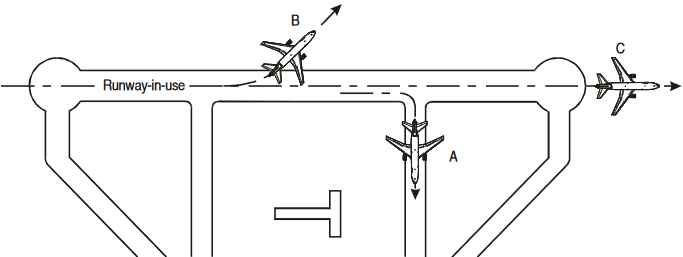
\includegraphics[width=0.8\textwidth]{4444/fig7-3.png}
    \caption{Separation between departing and arriving aircraft~\cite{4444}}
    \label{fig:separation_between_dep_and_arr}
\end{figure}

\clearpage
Separation of departing aircraft:
\begin{itemize}
    \item based on a surveillance system:
    \begin{itemize}
        \item 3~NM --- departures in different directions/different SIDs,
        \item 5~NM --- departures in the same direction/same SIDs,
        \item 5~NM --- departures in different directions/different SIDs, when the preceeding aircraft is 40~kts or more slower than the succeeding aircraft,
    \end{itemize}
    \item based on time:
    \begin{itemize}
        \item 5~minutes --- between departing aircraft on the same track, if the following aircraft will be crossing the level of the preceeding aircraft,
        \begin{figure}[htbp]
            \centering
            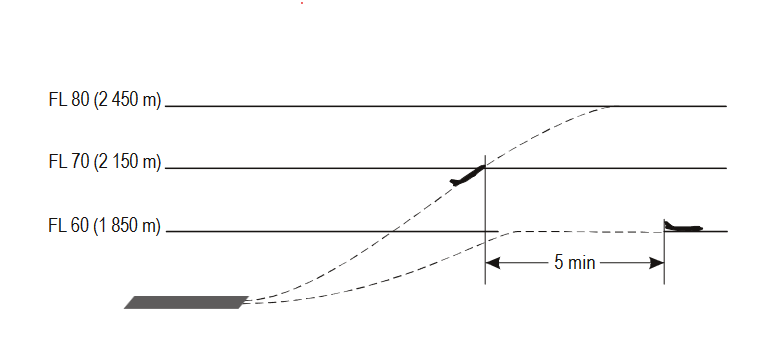
\includegraphics[width=0.5\textwidth]{4444/fig5-37.png}
            \caption{Five-minute separation of departing aircraft following the same track~\cite{4444}}
            \label{fig:5min_departures}
        \end{figure}
        \item 2~minutes --- between departing aircraft on the same track, when the preceeding aircraft is at least 40 kts faster,
        \begin{figure}[htbp]
            \centering
            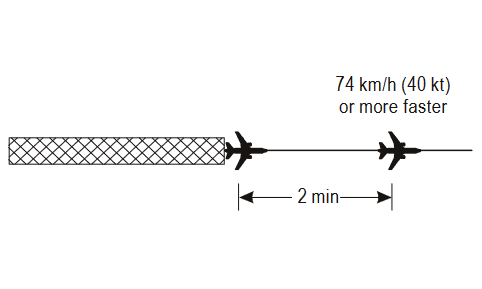
\includegraphics[width=0.5\textwidth]{4444/fig5-36.png}
            \caption{Two-minute separation between aircraft following same track~\cite{4444}}
            \label{fig:2min_departures}
        \end{figure}
        \item 1~minute --- between departing aircraft, when their departure tracks differ by no less than 45\degree ,
        \begin{figure}[htbp]
            \centering
            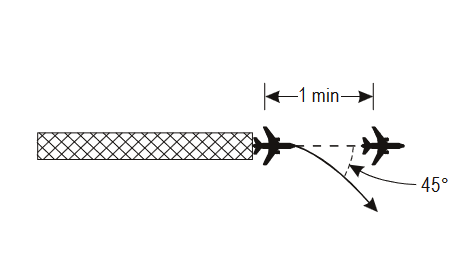
\includegraphics[width=0.5\textwidth]{4444/fig5-35.png}
            \caption{One-minute separation between departing aircraft following tracks diverging by at least 45\degree~\cite{4444}}
            \label{fig:1min_departures}
        \end{figure}
    \end{itemize}
    \item based on visual observation \emph{(VFR)}:
    \begin{itemize}
        \item aircraft has started a turn or passed departure end of the runway.
    \end{itemize}
\end{itemize}

Departures from intersecting runways are subject to common departure separations (requires usage of same separations as departures from the same runway).